\pagebreak
\subsubsection{UC15-Visualizzazione lista ristoranti}
\begin{figure}[h] 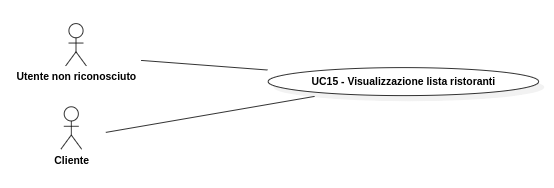
\includegraphics[scale=1]{uc15.png} \end{figure}
\begin{itemize}
\item \textbf{Attore principale:} Utente non riconosciuto / Cliente;
\item \textbf{Precondizioni:} L'utente è connesso al sistema;
\item \textbf{Postcondizioni:} L'utente visualizza una lista di ristoranti;
\item \textbf{Scenario principale:}
\begin{enumerate}
    \item L'utente seleziona la funzionalità di visualizzazione di una lista di ristoranti;
    \item L'utente visualizza una lista di ristoranti, ordinati secondo la loro valutazione media in ordine decrescente;
    \item Il sistema mostra per ogni ristorante queste informazioni:
       \begin{itemize}
           \item Il nome del ristorante;
           \item La tipologia/e di cucina del ristorante;
           \item La valutazione media ed il numero di valutazioni;
           \item Gli orari di apertura per la giornata di oggi o l'eventuale chiusura.
       \end{itemize}
\end{enumerate}
\end{itemize}

\pagebreak
\subsubsection{UC16-Ricerca ristorante}
\begin{figure}[h] 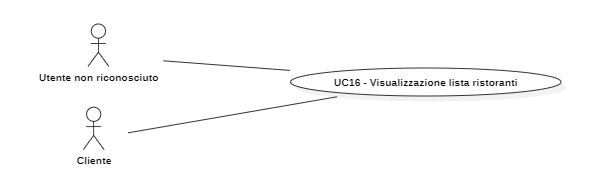
\includegraphics[scale=.7]{uc16.png} \end{figure}
\begin{itemize}
\item \textbf{Attore principale:} Utente non riconosciuto / Cliente;
\item \textbf{Precondizioni:} L'utente è connesso al sistema;
\item \textbf{Postcondizioni:} L'utente visualizza la lista dei ristoranti corrispondenti ai criteri inseriti dell'utente;
\item \textbf{Scenario principale:}
\begin{enumerate}
    \item L'utente seleziona la funzionalità di ricerca di un ristorante;
    \item L'utente può effettuare la ricerca inserendo uno o più parametri, corrispondenti ai seguenti criteri:
    \begin{itemize}
        \item Il nome del ristorante (vedi UC16.1-Ricerca per nome);
        \item La città del ristorante (vedi UC16.2-Ricerca per città);
        \item La valutazione media del ristorante (vedi UC16.3-Ricerca per valutazione);
        \item La tipologia di cucina (vedi UC16.4-Ricerca per tipologia di cucina);
        \item L'orario (vedi UC16.5-Ricerca ristorante per orario);
        \item La data (vedi UC16.6-Ricerca ristorante per data).
    \end{itemize}
    \item Il sistema filtra la lista di ristoranti secondo i criteri inseriti;
    \item L'utente visualizza la lista dei ristoranti che rispettano i criteri da lui inseriti.
\end{enumerate}
\end{itemize}

\pagebreak
\textbf{UC16.1-Ricerca ristorante per nome}
\begin{itemize}
\item \textbf{Attore principale:} Utente non riconosciuto / Cliente;
\item \textbf{Precondizioni:} L'utente è connesso al sistema;
\item \textbf{Postcondizioni:} L'utente visualizza la lista dei ristoranti corrispondenti alla ricerca per nome da lui inserito;
\item \textbf{Scenario principale:}
\begin{enumerate}
    \item L'utente seleziona la funzionalità di ricerca di un ristorante;
    \item L'utente inserisce il testo che deve essere contenuto nel nome;
    \item Il sistema filtra la lista di ristoranti secondo il criterio inserito;
    \item L'utente visualizza la lista dei ristoranti corrispondenti al nome da lui inserito.
\end{enumerate}
\end{itemize}

\textbf{UC16.2-Ricerca ristorante per città}
\begin{itemize}
\item \textbf{Attore principale:} Utente non riconosciuto / Cliente;
\item \textbf{Precondizioni:} L'utente è connesso al sistema;
\item \textbf{Postcondizioni:} L'utente visualizza la lista dei ristoranti corrispondenti alla città da lui inserita;
\item \textbf{Scenario principale:}
\begin{enumerate}
    \item L'utente seleziona la funzionalità di ricerca di un ristorante;
    \item L'utente inserisce la città come parametro di ricerca;
    \item Il sistema filtra la lista di ristoranti secondo il criterio inserito;
    \item L'utente visualizza la lista dei ristoranti corrispondenti alla città inserita.
\end{enumerate}
\end{itemize}

\textbf{UC16.3-Ricerca ristorante per valutazione}
\begin{itemize}
\item \textbf{Attore principale:} Utente non riconosciuto / Cliente;
\item \textbf{Precondizioni:} L'utente è connesso al sistema;
\item \textbf{Postcondizioni:} L'utente visualizza la lista dei ristoranti la cui valutazione è maggiore o uguale alla valutazione da lui inserita;
\item \textbf{Scenario principale:}
\begin{enumerate}
    \item L'utente seleziona la funzionalità di ricerca di un ristorante;
    \item L'utente inserisce il valore della valutazione che desidera;
    \item Il sistema filtra la lista di ristoranti secondo il criterio inserito;
    \item L'utente visualizza la lista dei ristoranti con valutazione maggiore o uguale a quella da lui inserita.
\end{enumerate}
\end{itemize}

\pagebreak

\textbf{UC16.4-Ricerca ristorante per tipologia di cucina}
\begin{itemize}
\item \textbf{Attore principale:} Utente non riconosciuto / Cliente;
\item \textbf{Precondizioni:} L'utente è connesso al sistema;
\item \textbf{Postcondizioni:} L'utente visualizza la lista dei ristoranti che offrono la tipologia di cucina da lui inserita;
\item \textbf{Scenario principale:}
\begin{enumerate}
    \item L'utente seleziona la funzionalità di ricerca di un ristorante;
    \item L'utente seleziona una o più tipologie di cucina alle quali è interessato;
    \item Il sistema filtra la lista di ristoranti secondo il criterio inserito;
    \item L'utente visualizza la lista dei ristoranti che offrono la/e tipologia/e di cucina da egli cercata.
\end{enumerate}
\end{itemize}

\textbf{UC16.5-Ricerca ristorante per orario}
\begin{itemize}
\item \textbf{Attore principale:} Utente non riconosciuto / Cliente;
\item \textbf{Precondizioni:} L'utente è connesso al sistema;
\item \textbf{Postcondizioni:} L'utente visualizza la lista dei ristoranti che hanno posti disponibili nell'orario da lui scelto;
\item \textbf{Scenario principale:}
\begin{enumerate}
    \item L'utente seleziona la funzionalità di ricerca di un ristorante;
    \item L'utente seleziona l'orario;
    \item Il sistema filtra la lista di ristoranti secondo il criterio inserito;
    \item L'utente visualizza la lista dei ristoranti che hanno posti disponibili nell'orario da lui selezionato.
\end{enumerate}
\end{itemize}

\textbf{UC16.6-Ricerca ristorante per data}
\begin{itemize}
\item \textbf{Attore principale:} Utente non riconosciuto / Cliente;
\item \textbf{Precondizioni:} L'utente è connesso al sistema;
\item \textbf{Postcondizioni:} L'utente visualizza la lista dei ristoranti che hanno posti disponibili nella data da lui selezionata;
\item \textbf{Scenario principale:}
\begin{enumerate}
    \item L'utente seleziona la funzionalità di ricerca di un ristorante;
    \item L'utente seleziona la data;
    \item Il sistema filtra la lista di ristoranti secondo il criterio inserito;
    \item L'utente visualizza la lista dei ristoranti che hanno posti disponibili nella data selezionata.
\end{enumerate}
\end{itemize}

\pagebreak
\subsubsection{UC17-Visualizzazione ristorante}
\begin{figure}[h] 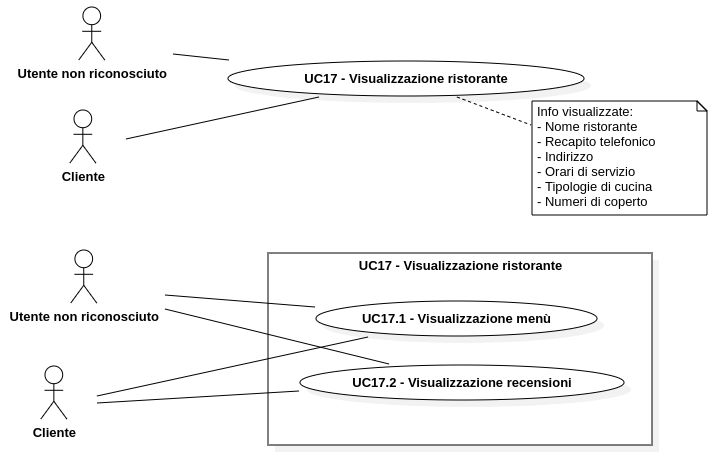
\includegraphics[scale=0.6]{uc17.png} \end{figure}
\begin{itemize}
\item \textbf{Attore principale:} Utente non riconosciuto / Cliente;
\item \textbf{Precondizioni:} L'utente è connesso al sistema e sta visualizzando una lista di ristoranti;
\item \textbf{Postcondizioni:} L'utente visualizza le informazioni relative al ristorante selezionato;
\item \textbf{Scenario principale:}
\begin{enumerate}
    \item L'utente seleziona un ristorante dalla lista che sta visualizzando;
    \item L'utente visualizza le informazioni relative al ristorante:
    \begin{itemize}
        \item Il nome;
        \item Il recapito telefonico;
        \item L'indirizzo;
        \item Gli orari di servizio;
        \item La/le tipologie di cucine offerte;
        \item Il numero di \emph{coperti}$^{G}$;
        \item La valutazione media.
    \end{itemize}
    \item L'utente può scegliere di visualizzare il menù completo (vedi UC17.1-Visualizzazione menù);
    \item L'utente può scegliere di visualizzare le recensioni rilasciate da altri utenti (vedi UC17.2-Visualizzazione recensioni).
\end{enumerate}
\end{itemize}

\pagebreak
\textbf{UC17.1-Visualizzazione menù}
\begin{itemize}
\item \textbf{Attore principale:} Utente non riconosciuto / Cliente;
\item \textbf{Precondizioni:} L'utente sta visualizzando le informazioni di un ristorante;
\item \textbf{Postcondizioni:} L'utente visualizza il menù del ristorante;
\item \textbf{Scenario principale:}
\begin{enumerate}
    \item L'utente seleziona la funzionalità di visualizzazione del menù del ristorante;
    \item L'utente visualizza la lista completa delle pietanze presenti nel menù;
    \item L'utente può effettuare la ricerca di una pietanza (vedi UC53-Ricerca pietanza);
    \item L'utente può visualizzare i dettagli relativi ad una singola pietanza presente nel menù (vedi UC17.1.2-Visualizzazione pietanza).
\end{enumerate}
\end{itemize}

\subsubsection{UC53-Ricerca pietanza}
\begin{figure}[h] 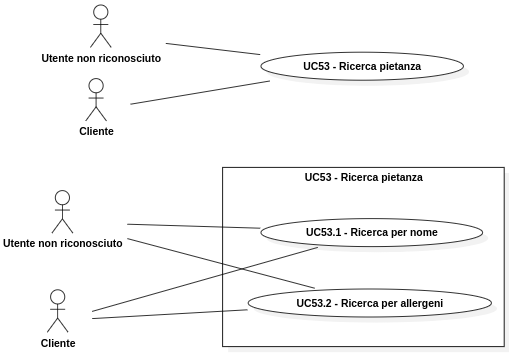
\includegraphics[scale=0.6]{uc53.png} \end{figure}
\begin{itemize}
\item \textbf{Attore principale:} Utente non riconosciuto / Cliente;
\item \textbf{Precondizioni:} L'utente sta visualizzando il menù di un ristorante;
\item \textbf{Postcondizioni:} L'utente visualizza la lista delle pietanze corrispondenti ai parametri di ricerca;
\item \textbf{Scenario principale:}
\begin{enumerate}
    \item L'utente seleziona la funzionalità di ricerca di una pietanza;
    \item L'utente può effettuare la ricerca per nome;
    \item L'utente può effettuare la ricerca selezionando gli allergeni che non vuole siano presenti nelle pietanze del menù;
    \item Il sistema filtra la lista delle pietanze secondo i parametri inseriti;
    \item L'utente visualizza la lista delle pietanze corrispondenti ai criteri di ricerca (la lista eventualmente può essere vuota).
\end{enumerate}
\end{itemize}

\textbf{UC17.1.2-Visualizzazione pietanza}
\begin{itemize}
\item \textbf{Attore principale:} Utente non riconosciuto / Cliente;
\item \textbf{Precondizioni:} L'utente sta visualizzando il menù di un ristorante;
\item \textbf{Postcondizioni:} L'utente visualizza le informazioni relative alla pietanza selezionata;
\item \textbf{Scenario principale:}
\begin{enumerate}
    \item L'utente seleziona una pietanza in particolare, presente nel menù che sta visualizzando;
    \item L'utente visualizza le seguenti informazioni ad essa relativa:
    \begin{itemize}
        \item La lista degli ingredienti in essa presenti;
        \item La lista degli allergeni;
        \item Il prezzo.
    \end{itemize}
\end{enumerate}
\end{itemize}

\pagebreak
\textbf{UC17.2-Visualizzazione lista recensioni}
\begin{itemize}
\item \textbf{Attore principale:} Utente non riconosciuto / Cliente;
\item \textbf{Precondizioni:} L'utente sta visualizzando le informazioni relative ad un ristorante;
\item \textbf{Postcondizioni:} L'utente visualizza le ultime 5 recensioni fatte in ordine temporale decrescente da altri utenti;
\item \textbf{Scenario principale:}
\begin{enumerate}
    \item L'utente seleziona la funzionalità di visualizzazione delle recensioni fatte da altri utenti sulla loro esperienza presso il ristorante;
    \item Il sistema presenta una lista con tutte le recensione di quel ristorante in ordine temporale decrescente;
    \item L'utente visualizza le seguenti informazioni per ogni recensione:
    \begin{itemize}
        \item Il nome del profilo che l'ha rilasciata;
        \item La data di rilascio;
        \item Un voto da 1 a 5 sul menù;
        \item Un voto da 1 a 5 sul servizio;
        \item Un voto da 1 a 5 sul prezzo;
        \item Un eventuale commento testuale.
    \end{itemize}
\end{enumerate}
\end{itemize}

\subsubsection{UC18-Prenotazione di un tavolo}
\begin{figure}[h] 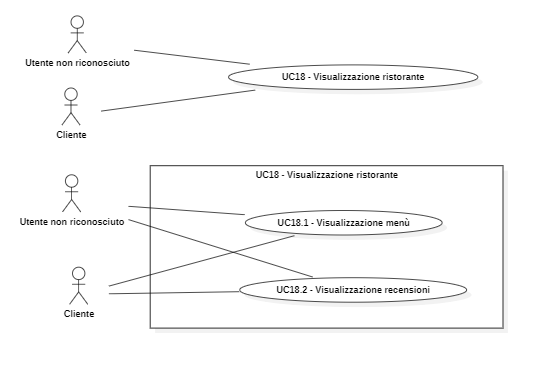
\includegraphics[scale=1]{uc18.png} \end{figure}
\begin{itemize}
    \item \textbf{Attore principale:} Cliente;
    \item \textbf{Precondizioni:} Il cliente sta visualizzando le informazioni di un ristorante;
    \item \textbf{Postcondizioni:} La prenotazione è salvata nella lista delle prenotazioni del cliente;
    \item \textbf{Scenario principale:}
        \begin{enumerate}
            \item Il cliente seleziona la funzionalità di richiesta di una nuova prenotazione;
            \item Il sistema illustra i giorni in cui è possibile effettuare la richiesta;
            \item Il cliente seleziona il giorno di calendario;
            \item Il sistema illustra le fasce orarie disponibili;
            \item Il cliente seleziona l'orario;
            \item Il cliente inserisce il numero di persone che parteciperanno alla prenotazione;
            \item Il cliente dà la conferma ed effettua la richiesta;
            \item Il cliente visualizza la lista delle sue prenotazioni, ove è presente la prenotazione appena effettuata.
        \end{enumerate}
\end{itemize}

\pagebreak
\subsubsection{UC19-Visualizzazione lista prenotazioni} % UC19: Deve essere modellata come una lista di informazioni
\begin{figure}[h] 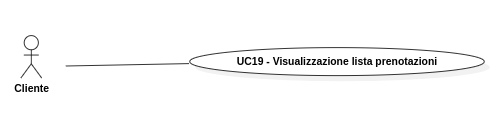
\includegraphics[scale=1]{uc19.png} \end{figure}
\begin{itemize}
    \item \textbf{Attore principale:} Cliente;
    \item \textbf{Precondizioni:} L'utente ha selezionato un profilo cliente;
    \item \textbf{Postcondizioni:} Il cliente visualizza la lista delle sue prenotazioni;
    \item \textbf{Scenario principale:}
        \begin{enumerate}
            \item Il cliente seleziona la funzionalità di visualizzazione delle sue prenotazioni;
            \item Il cliente può filtrare le prenotazioni tramite dei parametri (si veda UC15);
            \item Il cliente può selezionare una prenotazione singola per vederne il dettaglio (si veda UC21);
            \item Il cliente visualizza le seguenti informazioni per ogni prenotazione:
              \begin{itemize}
                \item Il ristorante;
                \item La timestamp per cui è programmata;
                \item Il numero di persone partecipanti;
                \item Lo stato (In Attesa, Accettata, Rifiutata).
              \end{itemize}
        \end{enumerate}
\end{itemize}

\subsubsection{UC20-Filtra prenotazioni}
\begin{figure}[h] 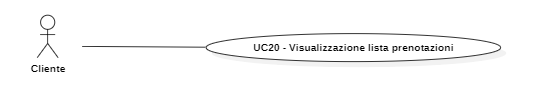
\includegraphics[scale=1]{uc20.png} \end{figure}
\begin{itemize}
\item \textbf{Attore principale:} Cliente;
\item \textbf{Precondizioni:} Il cliente sta visualizzando la lista delle sue prenotazioni;
\item \textbf{Postcondizioni:} Il cliente visualizza la lista delle prenotazioni corrispondenti ai parametri di filtraggio;
\item \textbf{Scenario principale:}
\begin{enumerate}
    \item Il cliente seleziona l'opzione di filtraggio delle prenotazioni;
    \item Il cliente può filtrare le prenotazioni secondo i parametri:
              \begin{itemize}
                \item Range temporale: Data di inizio e data di fine;
                \item Stato: "In Attesa", "Accettata" o "Rifiutata".
              \end{itemize}
    \item Il sistema filtra la lista di prenotazioni secondo il parametro selezionato;
    \item Il cliente visualizza la lista di prenotazioni corrispondenti al parametro da lui selezionato.
\end{enumerate}
\end{itemize}

\subsubsection{UC21-Visualizzazione singola prenotazione}
\begin{figure}[h] 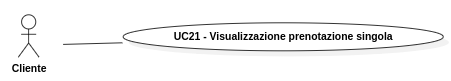
\includegraphics[scale=1]{uc21.png} \end{figure}
\begin{itemize}
    \item \textbf{Attore principale:} Cliente;
    \item \textbf{Attore secondario:} Ristoratore;
    \item \textbf{Precondizioni:} Il cliente sta visualizzando la lista delle sue prenotazioni;
    \item \textbf{Postcondizioni:} Il cliente visualizza le informazioni relative ad una singola prenotazione;
    \item \textbf{Scenario principale:}
        \begin{enumerate}
            \item Il cliente seleziona una prenotazione in particolare;
            \item Il cliente visualizza la lista delle informazioni relative alla prenotazione selezionata:
            \begin{itemize}
                \item Il nome del ristorante;
                \item L'indirizzo del ristorante;
                \item L'orario;
                \item Il numero di persone;
                \item Lo stato della prenotazione (se è in attesa di accettazione da parte del ristoratore o se è già stata accettata);
            \item Il cliente può andare a generare il link per la condivisione della prenotazione (si veda UC23).
            \end{itemize}
        \end{enumerate}
\end{itemize}

\pagebreak
\subsubsection{UC22-Cancellazione prenotazione}
\begin{figure}[h] 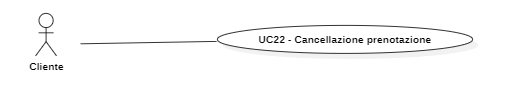
\includegraphics[scale=1]{uc22.png} \end{figure}
\begin{itemize}
    \item \textbf{Attore principale:} Cliente;
    \item \textbf{Precondizioni:} Il cliente sta visualizzando le informazioni di una singola prenotazione e c'è una differenza di almeno 48 ore tra il datetime in cui il cliente fa la richiesta di cancellazione e quello della prenotazione;
    \item \textbf{Postcondizioni:} La prenotazione è stata cancellata e non è più presente nella lista di prenotazioni del cliente;
    \item \textbf{Scenario principale:}
        \begin{enumerate}
            \item Il cliente seleziona l'opzione di cancellazione della prenotazione;
            \item Il cliente dà la conferma ed effettua la cancellazione;
            \item Il sistema notifica il ristoratore dell'avvenuta cancellazione;
            \item Il cliente visualizza la lista delle sue prenotazioni aggiornata, priva di quella appena cancellata.
        \end{enumerate}
\end{itemize}

\subsubsection{UC23-Condivisione della prenotazione}
\begin{figure}[h] 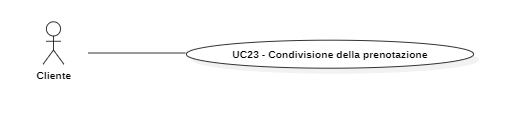
\includegraphics[scale=1]{uc23.png} \end{figure}
\begin{itemize}
    \item \textbf{Attore principale:} Cliente;
    \item \textbf{Precondizioni:} Il cliente sta visualizzando le informazioni di una sua singola prenotazione (si veda UC21);
    \item \textbf{Postcondizioni:} Il cliente ha una copia testuale del link relativo alla prenotazione;
    \item \textbf{Scenario principale:}
        \begin{enumerate}
            \item Il cliente seleziona la funzionalità di condivione del link afferente alla prenotazione;
            \item Il sistema genera il link relativo alla prenotazione;
            \item Il cliente visualizza il link di invito.
        \end{enumerate}
\end{itemize}

\pagebreak
\subsubsection{UC24-Accettazione di invito di partecipazione ad una prenotazione}
\begin{figure}[h] 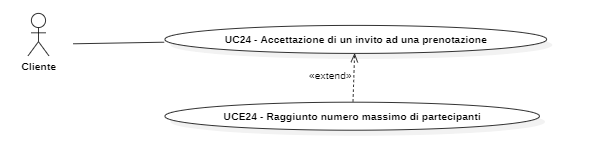
\includegraphics[scale=.7]{uc24.png} \end{figure}
\begin{itemize}
    \item \textbf{Attore principale:} Utente non riconosciuto;
    \item \textbf{Precondizioni:} L'utente possiede il link per partecipare ad una prenotazione;
    \item \textbf{Postcondizioni:} La prenotazione è salvata nella lista delle prenotazioni dell'utente;
    \item \textbf{Scenario principale:}
        \begin{enumerate}
            \item L'utente seleziona il link di partecipazione alla prenotazione;
            \item L'utente effettua il login per accedere al sistema;
            \item L'utente seleziona il profilo cliente con il quale partecipare alla prenotazione;
            \item L'utente visualizza la prenotazione alla quale è stato invitato nella lista delle sue prenotazioni.
        \end{enumerate}
        \item \textbf{Estensione:} UCE24-Raggiunto numero massimo di partecipanti.
    \end{itemize}

\subsubsection{UCE24-Raggiunto numero massimo di partecipanti}
\begin{itemize}
    \item \textbf{Descrizione:} Possono accedere alla prenotazione tramite il link di invito un numero massimo di utenti uguale al numero di partecipanti indicato al momento della prenotazione;
    \item \textbf{Scenario alternativo:}
    \begin{enumerate}
        \item L'utente riconosciuto seleziona il profilo con il quale partecipare alla prenotazione;
        \item Il sistema notifica all'utente un messaggio di errore, in cui gli comunica che è stato già raggiunto il numero massimo di partecipanti; %Forse l'estensione può terminare anche con il messaggio di errore;
        \item L'utente visualizza la sua lista di prenotazioni senza la prenotazione alla quale voleva partecipare.
    \end{enumerate}
\end{itemize}

